\chapter{Feature Matching}
\label{sec:matching}
Once the interest points have been detected and the descriptors have been computed, the interest points can be matched between pairs of images. This is achieved by first calculating the distance in feature space between the interest point descriptors in each image. The interest points are then matched if their descriptor distances are within various thresholds or constraints of one another as pre-defined by the matching technique that is being utilised. An example of matches found from comparing a pair of images is shown in \figref{fig:matchesIntro}. Matched interest points in corresponding images are connected by a green line as seen in the figure. Interest points that have not been matched are represented by red circles.\\

\begin{figure}[h!] 
  \centering
    \includegraphics[width=0.8\textwidth]{../Drawings/brisk/matches.jpg}
    \caption{An example of matches between a pair of images. The matches are connected by green lines.}
    \label{fig:matchesIntro}
\end{figure}

The methods used to calculate the distance between interest point descriptors will be detailed. The various constraints imposed to determine whether a match between two interest points is indeed valid will be described in \secref{sec:validation}. In addition to this, the various matching techniques utilised to match interest points will also be detailed in \secref{sec:matchingTechniques}.\\

\section{Calculating Distance between Feature Descriptors}
\label{sec:distance}

\subsection{Hamming Distance}
\label{sec:hamming}
The Hamming distance is a measure of the distance between two strings \citep{Banzal2007}. The distance between two strings is defined as the number of corresponding bits, letters or numbers that differ between these strings. Assume that there are two strings $A$ and $B$ of equal length. In this example, these strings can only take values of $0$ or $1$. The hamming distance is then calculated by determining whether or not the values of corresponding elements in each of the strings are different. If the values are different, then the hamming distance is incremented by a value of $1$.\\

This metric is used to determine the distance between feature descriptors in the BRISK algorithm \citep{Leutenegger2011}. Since the feature descriptors, as mentioned in \secref{sec:briskDescribe}, are vectors of $512$ bits in length, the Hamming distance of two feature descriptors is calculated by determining how different the first feature descriptor is from the second. The bits can only take values of $0$ or $1$. It is desired that the feature descriptors are as similar as possible for the descriptors to be a match; that is, they have a very low hamming distance value. \\

This is a very efficient algorithm and has been effectively performed in BRIEF \citep{Calonder}. It consists of $512$ XOR operations between corresponding bits followed by a bit count. This is a very efficient computation to perform on modern day architectures \citep{Leutenegger2011}. \\ 

\subsection{Euclidean Distance}
\label{sec:euclidean}
In SURF-based approaches,  the Euclidean distance is used as a metric to determine whether or not there is a match between two feature descriptors \citep{Lowe2004}. Given two feature descriptors of length $64$, the Euclidean distance is calculated between descriptors in feature space and results in a value indicating the difference between the two feature descriptors. As in BRISK, it is desired that the Euclidean distance is as small as possible between the descriptors for them to be a match. A match occurs if the nearest neighboring feature descriptor corresponding to an interest point in image $A$ is within a specified euclidean distance from the descriptor of the corresponding matched interest point in image $B$.\\

In addition to this, in order to speed up matching, the sign of the Laplacian, which is the trace of the Hessian matrix, is used to determine whether or not each blob response in the respective images are of a similar contrast \citep{Bay2008}. The sign of the Laplacian determines whether the interest point in question is a dark blob on a light background or a light blob on a dark background. This enables interest points of different contrasts to be rejected as matches without having to compute the euclidean distance between the points.\\

\section{Validating Matched Features}
\label{sec:validation}
Once the hamming or euclidean distance is computed between two descriptors and the specified distance is within a pre-defined threshold, the corresponding interest points are considered to be a match. However, this match may not necessarily be a valid match and a number of constraints have been imposed in order to verify the match.\\

\subsection{2-Nearest Neighbors Ratio}
\label{sec:2nnMatching}
The 2-NN Ratio is computed using the closest and second closest match for a particular interest point \citep{Lowe2004}. The equation is shown in \eqnref{eqn:2nnRatio}. This constraint therefore requires that each interest point has at least two matches. This is performed for every detected interest point in the image being evaluated. It has been assumed that each interest point has only a single, unique corresponding match between a pair of images. Based on this assumption, the closest match should be the true matching interest point in the corresponding image, whereas the second closest match should belong to a different object in the image and hence is an invalid match.\\

\begin{equation}
Ratio_{2-NN} = \frac{\mbox{Closest Match}}{\mbox{Second Closest Match}}
\label{eqn:2nnRatio}
\end{equation}

Therefore, for a valid match between interest points, the closest match should be significantly closer than the second closest match (which is the closest incorrect match) from the interest point that is being evaluated \citep{Lowe2004}. This means that a valid match should generally have a lower 2-NN ratio than an invalid match. An invalid match will probably have a number of matches within a similar distance of one another due to the high dimensionality of the feature space \citep{Lowe2004}. The feature space, as mentioned previously is of dimensionality $64$ for 2D SURF and $512$ for BRISK-based techniques.\\

Based on the results in \secref{sec:knnMatchingConstraint}, all matches with a threshold above $0.7$ are rejected as invalid matches whereas all matches with a threshold below this value are accepted as valid matches. An example of the 2-NN constraint can be seen in \figref{fig:2nn_1} and \figref{fig:2nn_2}. \figref{fig:2nn_1} shows the interest points in the left image where each interest point has two matches in the right image. After applying the 2-NN ration constraint, a number of invalid matches are discarded and the best match for each interest point is displayed  as seen in \figref{fig:2nn_2}.\\


\begin{figure}[h!] 
  \centering
    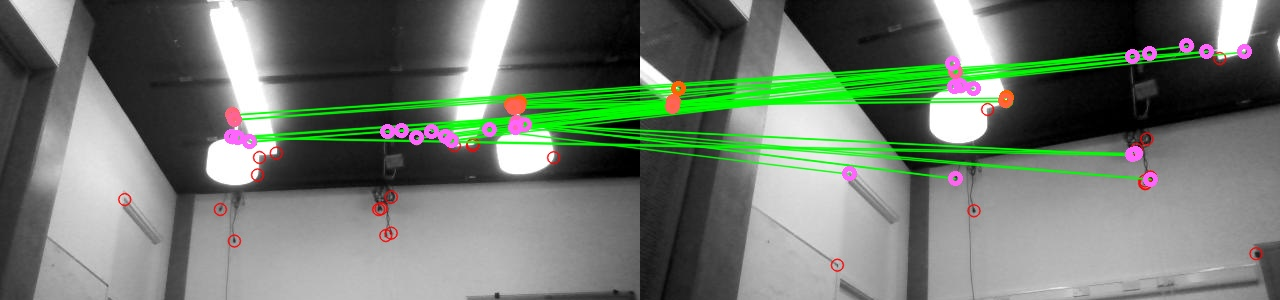
\includegraphics[width=0.8\textwidth]{../Drawings/Matching/feature_matching/dataset_2nn_matching_constraint_before.jpg}
    \caption{Matched interest points before applying the 2-NN ratio constraint}
    \label{fig:2nn_1}
\end{figure}

\begin{figure}[h!] 
  \centering
    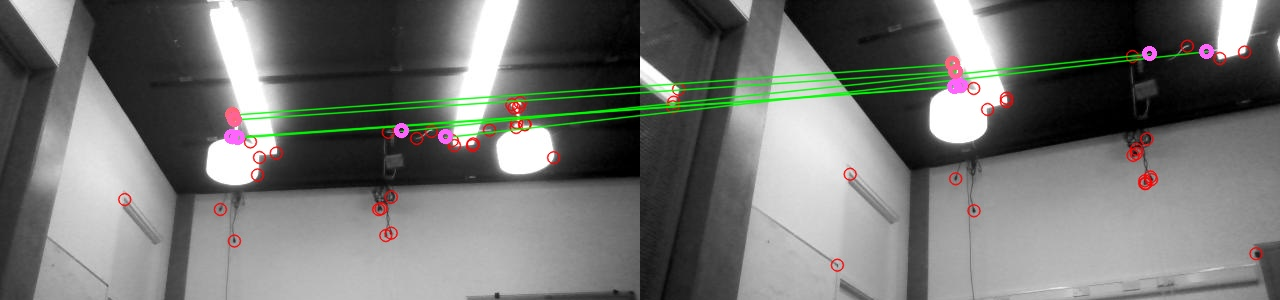
\includegraphics[width=0.8\textwidth]{../Drawings/Matching/feature_matching/dataset_2nn_matching_constraint_after.jpg}
    \caption{The best matches are displayed after having applied the 2-NN ratio constraint}
    \label{fig:2nn_2}
\end{figure}


\subsection{Angle and Distance Constraints}
\label{sec:angleDistanceConstraints}
Two additional matching constraints have been developed in order to determine whether or not a match between two interest points in corresponding images are valid; namely, the angle and distance constraints respectively. A pair of interest points have to fulfil both of these constraints in order to be considered a valid match. In order to verify that the match fulfils these constraints, the pair of images that are being evaluated are placed next to one another as shown in \figref{fig:angleConstraint}. A line is then connected between each pair of matched interest points as shown in \figref{fig:angleConstraint} and \figref{fig:distanceConstraint}. It is this line that is used to determine whether the matched pair of interest points are valid.\\

The angle constraint calculates the angle from the interest point in the left image relative to the interest point in the right image. It has been determined through visual analysis that the angle between two matched interest points should be less than  $10^{\circ}$. This is because corresponding matches should be placed at approximately the same height provided there are no large image rotations. Since Robocup is the immediate application, negligible rotation is expected as the robot re-enters the field after a \textit{Standard Removal Penalty}.
If the angle is within the pre-defined threshold then the match is valid, otherwise it is invalid. As can be seen in the figure, $\alpha$ is larger than the pre-defined threshold and therefore the match is marked as invalid. $\beta$ is within the threshold and therefore pertains to a valid match. \\

The distance constraint states that the length of the line connecting two matched interest points should be the width of the image plus a pre-defined threshold. This constraint assumes no significant scale changes which is again feasible based on the current application domain. A pre-defined threshold of $200$ pixels has been chosen based in visual analysis. As can be seen in \figref{fig:distanceConstraint}, the longer line does not pass the distance constraint and is marked as being invalid.\\

\begin{figure}[ht!]
\begin{minipage}[b]{0.5\linewidth}
  \centering
    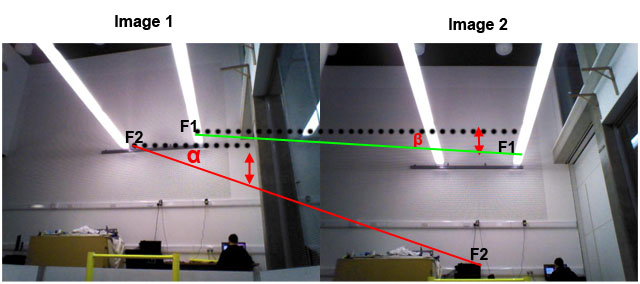
\includegraphics[width=1.0\textwidth]{../Drawings/constraints/angleConstraintMerged.jpg}
    \caption{The angle constraint that has been developed to remove invalid matches} 
    \label{fig:angleConstraint}
\end{minipage}
\begin{minipage}[b]{0.5\linewidth}
  \centering
    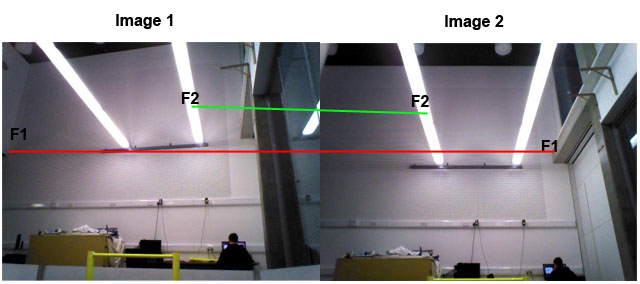
\includegraphics[width=1.0\textwidth]{../Drawings/constraints/distanceConstraint.jpg}
    \caption{The distance constraint that has been developed to remove invalid matches} 
    \label{fig:distanceConstraint}
\end{minipage}
\end{figure}

%\begin{figure}[h!] 
%  \centering
%    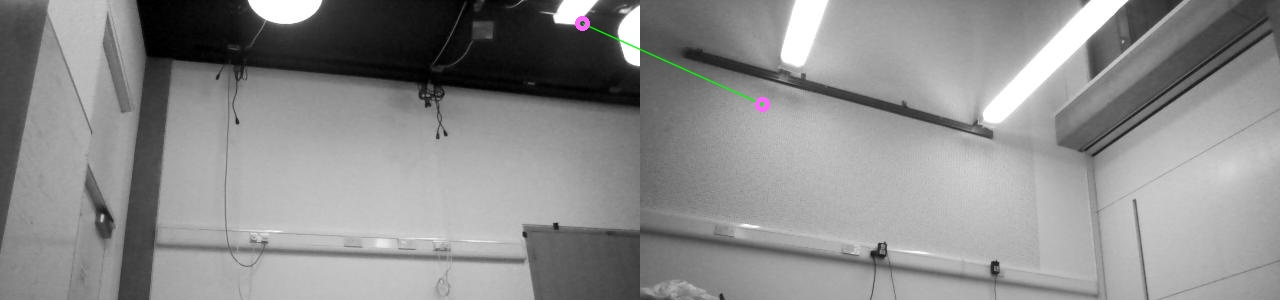
\includegraphics[width=0.8\textwidth]{../Drawings/constraints/t_20_hd_55_OG_Left_MG_Right_2_12.jpg}
%    \caption{An incorrect match detected due to an angle larger than $10^\circ$}
%    \label{fig:imagesSide}
%\end{figure}


\section{Feature Matching Techniques}
\label{sec:matchingTechniques}
Three main feature matching techniques have been utilised in this thesis. Both BRISK and 2D SURF-based approaches make use of 2-Nearest Neighbors and Radius Matching. A matching technique called Nearest Neighbors with RANSAC has been developed by the \textit{rUNSWift} Robocup team \citep{Anderson}. This technique is used for the 1D SURF feature extraction algorithm. These feature matching techniques assume that interest points with corresponding feature descriptors in image $A$ (query image) are being compared to interest points with their corresponding descriptors in image $B$ (stored image). \\

\subsection{2-Nearest Neighbours Matching}
\label{sec:knn}
The 2-Nearest Neighbors (2-NN) feature matching technique involves finding two interest points  in image $B$ that yield the closest matches to the interest point that is currently being evaluated in image $A$. This technique ensures that two matches will be found for every interest point in the query image $A$. Therefore the number of matches is always twice the total number of interest points in the query image.\\

The algorithm is implemented as follows. Initially, the interest points in both the stored and query images are detected. Their descriptors are computed and all of the descriptors in the query and stored image pair are sent into the 2-NN matching algorithm. The hamming/euclidean distance (depending on the method) between each query descriptor and all of the stored descriptors is then calculated. The top two stored descriptors yielding the lowest hamming/euclidean distance are assigned as matches to the query descriptor. These matches are stored in descending order where the first match has the lower of the two distances. An example of three interest points, in query image $A$, with two corresponding matches each, in the stored image $B$, is shown in \figref{fig:2nn_matching}. \figref{fig:2nn_best_match} shows the best match for each of the interest points.\\

It must be noted that both the 2-NN ratio constraint and the angle and distance constraints respectively are applied to this matching technique.\\

 \begin{figure}[h!] 
  \centering
    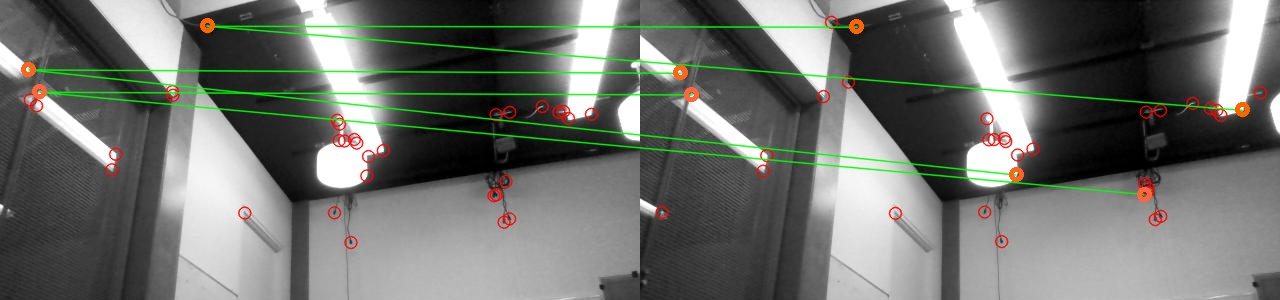
\includegraphics[width=0.8\textwidth]{../Drawings/Matching/feature_matching/dataset1_without_validation_knn.jpg}
    \caption{The interest points in the left image (image $A$) and their corresponding 2-NN matches in the right image (image $B$)}
    \label{fig:2nn_matching}
\end{figure}

 \begin{figure}[h!] 
  \centering
    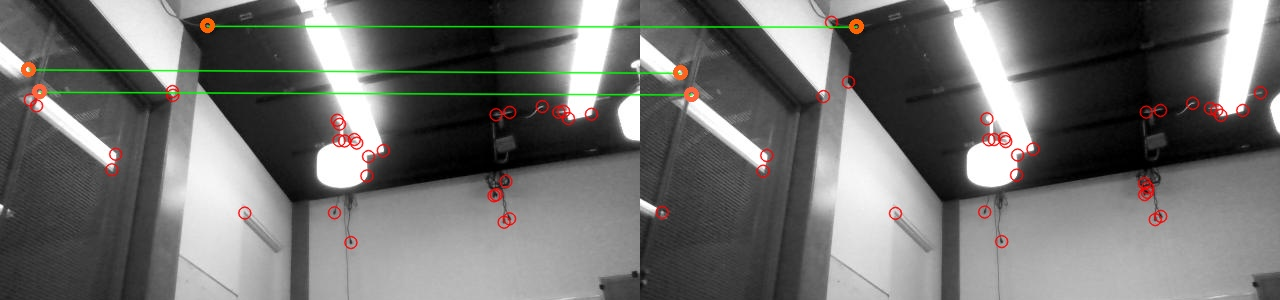
\includegraphics[width=0.8\textwidth]{../Drawings/Matching/feature_matching/dataset1_without_validation_knn_best.jpg}
    \caption{The best matched interest points}
    \label{fig:2nn_best_match}
\end{figure}

\subsection{Radius Matching}
\label{sec:radius}
Radius matching is different from 2-NN in that a match between a pair of interest points only occurs if the calculated hamming or euclidean distance (depending on the feature extraction algorithm being used) is below a pre-defined threshold. This threshold is denoted the `Hamming Distance' for BRISK-based algorithms and the `Euclidean Distance' for 2D SURF-based algorithms respectively. \\

This method does not guarantee that every interest point in the query image will have a corresponding match in the stored image. In contrast, this method does not limit the amount of matches that an interest point in the query image can generate.\\

The Radius Matching algorithm therefore computes the descriptors for all of the interest points in both the query and stored images respectively. The descriptors are then matched if the distance is below the pre-defined threshold. These matches are sorted and stored in descending order where the first match has the smallest Hamming/Euclidean distance. Matches generated from Radius Matching can be seen in \figref{fig:radius_match}. Here, one of the interest points in the query image has more than two matches with interest points in the stored image. The best matches for this pair of images is shown in \figref{fig:radius_best_match}.\\ 


 \begin{figure}[h!] 
  \centering
    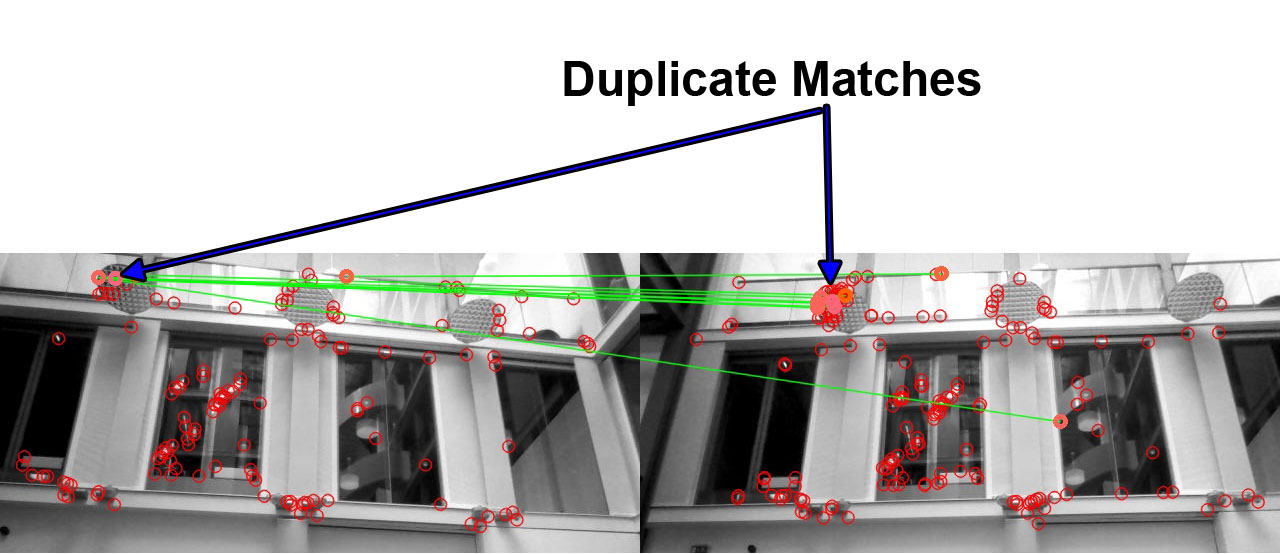
\includegraphics[width=0.8\textwidth]{../Drawings/Matching/feature_matching/dataset1_without_validation_radius_photo.jpg}
    \caption{Matched interest points due to Radius Matching. Note the interest point with more than two matches.}
    \label{fig:radius_match}
\end{figure}

 \begin{figure}[h!] 
  \centering
    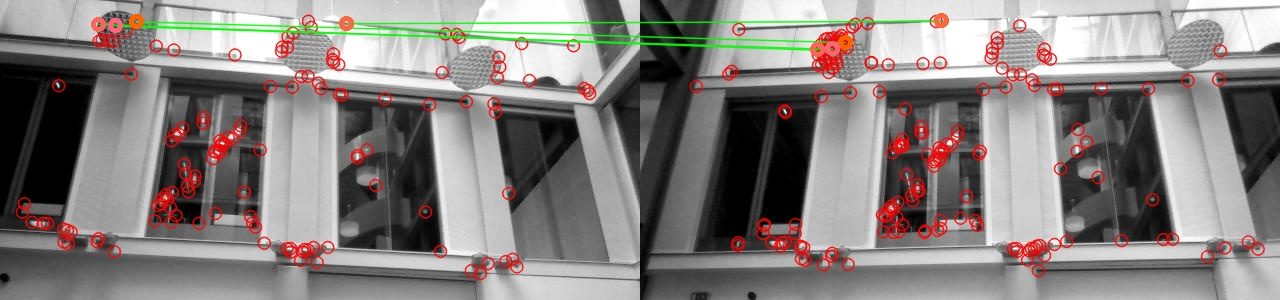
\includegraphics[width=0.8\textwidth]{../Drawings/Matching/feature_matching/dataset1_without_validation_radius_best.jpg}
    \caption{The best matched interest points using Radius Matching}
    \label{fig:radius_best_match}
\end{figure}

\subsection{RANSAC Matching}
\label{sec:ransacMatching}
The RANSAC matching technique has been developed for the 1D SURF implementation \citep{Anderson}. This technique is composed of two stages, namely Nearest Neighbors followed by RANSAC. The nearest neighbors stage calculates the distance in feature space from the first and second nearest neighbor to the interest point being evaluated. It then calculates the 2-NN ratio defined in \secref{sec:2nnMatching} to determine whether the match is indeed valid. The pre-defined threshold for this implementation is $0.75$.\\

Once this stage has been processed, the RANSAC procedure is initialised. This stage removes interest points that do not conform to a straight line function defined in \eqnref{eqn:straightLine} \citep{Anderson}. Here, $x_{query,i}$ is the x position of the $i^{th}$ matched interest point along a single row of pixels in the query image $A$.  $x_{stored,i}$ is the x position in the stored image $B$. $\beta_s$ and $\beta_d$ are scaling and displacement parameters.\\

\begin{equation}
x_{query,i} = \beta_s x_{stored,i} + \beta_d
\label{eqn:straightLine}
\end{equation} 

To illustrate the meaning of this function, consider \figref{fig:ransacOverview}. The query image $A$ is the bottom image and the stored image is the top left image. Note that the stored image has been rotated clockwise by $90^{\circ}$ for visualisation purposes. The single row of pixels used to detect features can be seen at the top of each image. The single row of pixels have been computed using the pixels within the two red bands in each image as described in \secref{sec:1dsurf}. The $i^{th}$ match generated from the 2-NN ratio is shown in \figref{fig:ransacExample}. The x position for each image is computed and placed into \eqnref{eqn:straightLine}. If $x_{query,i} - (\beta_s x_{stored,i} + \beta_d) \leq P$ where $P$ is a pre-defined threshold, then the interest points are a valid match. If the interest points are valid, then the inverse distance in feature space between the pair of interest points' feature descriptors is computed and is added to a scoring function. Invalid interest points are discarded. This procedure removes outliers and provides a score of how well a pair of images match one another \citep{Anderson}.\\


\begin{figure}[ht!]
\begin{minipage}[b]{0.5\linewidth}
  \centering
    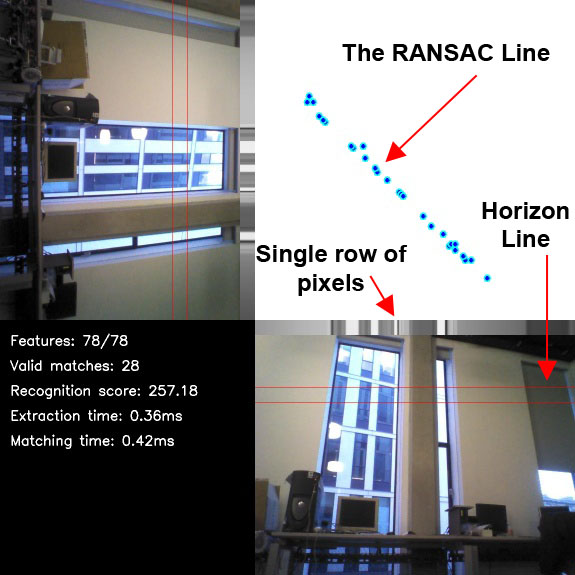
\includegraphics[width=0.8\textwidth]{../Drawings/constraints/matchingLabelled.jpg}
    \caption{An overview of the matching constraints imposed in the 1D SURF algorithm} 
    \label{fig:ransacOverview}
\end{minipage}
\begin{minipage}[b]{0.5\linewidth}
  \centering
    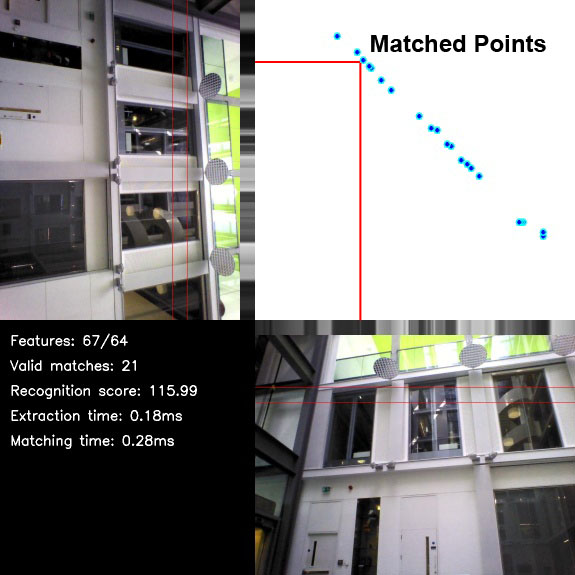
\includegraphics[width=0.8\textwidth]{../Drawings/constraints/matchedPoints.jpg}
    \caption{An example of how the matches are constructed} 
    \label{fig:ransacExample}
\end{minipage}
\end{figure}